%%%%%%%%%%%%%%%%%%%%%%%%%%%%%%%%%%%%%%%%%%%%%%%%%%%%%%%%%%%%%%%
%2345678901234567890123456789012345678901234567890123456789012345678901234567890
%        1         2         3         4         5         6         7         8

\documentclass[letterpaper, 10 pt, conference]{ieeeconf}  % Comment this line out if you need a4paper

%\documentclass[a4paper, 10pt, conference]{ieeeconf}      % Use this line for a4 paper

\IEEEoverridecommandlockouts                              % This command is only needed if 
                                                          % you want to use the \thanks command

\overrideIEEEmargins                                      % Needed to meet printer requirements.

% See the \addtolength command later in the file to balance the column lengths
% on the last page of the document

% The following packages can be found on http:\\www.ctan.org
\usepackage{graphicx} % for pdf, bitmapped graphics files
%\usepackage{epsfig} % for postscript graphics files
%\usepackage{mathptmx} % assumes new font selection scheme installed
%\usepackage{times} % assumes new font selection scheme installed
\usepackage{amsmath} % assumes amsmath package installed
\usepackage{amsfonts} % assumes amsfonts package installed
%\usepackage{amssymb}  % assumes amsmath package installed

\title{\LARGE \bf {Wavelet Based ROI Lossless Medical Image Watermarking Scheme}}


\author{\it Rui Shen, Pouria Tohidi, Shuwen Wei  \\ % <-this % stops a space
\normalsize {Department of Electrical and Computer Engineering, Johns Hopkins University}
\thanks{520.646 WAVELETS AND FILTER BANKS}}

\begin{document}



\maketitle
\thispagestyle{empty}
\pagestyle{empty}


%%%%%%%%%%%%%%%%%%%%%%%%%%%%%%%%%%%%%%%%%%%%%%%%%%%%%%%%%%%%%%%%%%%%%%%%%%%%%%%%
\begin{abstract}


\end{abstract}


%%%%%%%%%%%%%%%%%%%%%%%%%%%%%%%%%%%%%%%%%%%%%%%%%%%%%%%%%%%%%%%%%%%%%%%%%%%%%%%%
\section{INTRODUCTION}
% Background introduction, like where the problems are
As the amount of patient data becomes increasingly larger in the hospital system, it is important to find an efficient way to store, retrieve and distribute the data. Traditionally, the patient data is stored separately from the corresponding medical scanned image like CT images, MRI images and so on. However, mistakes may sometimes happen when a doctor tries to extract the corresponding patient data to match a certain medical scanned image. Furthermore, the confidentiality is not always good when the hospital system is attacked by the hostile people, which may finally lead to the leakage of patient information.

% Propose a solution, review the previous work on this field
One simple solution is to embed the patient information into the corresponding scanned medical images. In this way, a doctor can always extract the right patient inforamtion from the medical image. And even when the hospital system is attacked, the patient information embeded in the medical image is hard to decode as well. Furthermore, as the patient information is hidden in the medical image, it will save the strorage space especially when the amount of patient data becomes larger nowadays. Moreover, it becomes easlier to distribute the patient data especially in the application teletadiology which requires the medical images to be transmitted over the electronic networks for clinical interpretation, where the privacy and security are more important.

Watermarking, which is origially used for image authentication, now becomes a powerful tool in hiding the patient information into the medical scanned image. The application of watermarking is well established nowadays, and its potential in medical system information is being gradually recognized. Many works have been done in this field. In 2006, Dekun Zou et al. prposed a new semi-fragile lossless digital watermarking scheme, which use 5/3 filter bank thus can be easliy integrated into the JPEG 2000 standard. Also it takes special measures so that it does not suffer from the salt-and-pepper noise and the impact of the compression. In 2010, Malay Kumar Kundu et al. proposed a lossless region of interest (ROI) preserving medical image watermarking technique in spatial domain. It combined lossless data compresson and encryption techniques so that it will help maintain data privacy and image integrity. In 2011, A. Kannammal et al. proposed a fragile image authenticziton scheme for DICOM image based on discrete wavelet transform. By using some hybrid coding like Bose–Chaudhuri–Hocquenghem (BCH) encoded method, it performs better in source authentication, data authentication and transfer of patient data as well. Different attacks are used to test the watermarked image and the method still works well even when the image goes through rotation, flip or noising. In 2014, Mohamed Ali Hajjaji et al. combined Haar wavelet and Karhunen Loeve transform so that it extract information more accurately even under various types of attacks.

% Propose our method, and why it's better than the previous work or where is the innovation
In this paper, we proposed a watermarking method in wavelets domain to embed the patient data into the corresponding medical scanned image. First, we introduce a common watermarking skill in spatial domain. Then we propose a new watermarking algorithm based on wavelets domain, including the encoding part and decoding part. Finally, different attacks are applied to the watermarked images to prove the robustness of the algorithm and we compare the performance of the watermark in spatial domain and wavelets domain. In the encoding part, we apply a four level discrete Haar wavelets transform to the original medical image and use different block to store different kind of informaiton. For each block we have a special key which indicate the position where the information is stored. Also, by doing the segementation, we distinguish the region of non-interest (RONI) from the ROI in the medical scanned images and the real infromation is stored in the key from the RONI. Moreover, BCH encode is implemented to enable tamper detection. In the decoding part, we first use BCH to determine if there are any tamper or not. Then we use the key and the RONI segementation to retrieve the information from the wavelets domain.

\section{DATA}


\section{METHODOLOGY}
\subsection{Watermark embedding}
The EPR data was split into several blocks for embedding into different sub-bands of wavelet decomposition levels  (Fig. \ref{WMPos}). The energy of the image is mainly concentrated in the high decomposition level while the low frequency. Among sub-bands in the same level, the diagonal ones contain the least energy which means they are more vulnerable to attack. Embedding the watermark in the diagonal detail in the first level can be used in tamper assessing detection of the image. Compared with the diagonal sub-bands, the horizontal and the vertical ones include higher energy, which can guarantee increased robustness when storing EPR data. However, the coarse approximation contains the most crucial information of the original image and would significantly affect the image quality, this sub-bands should avoid any changing in wavelet coefficients.
\begin{figure}[htbp]
	\centering
	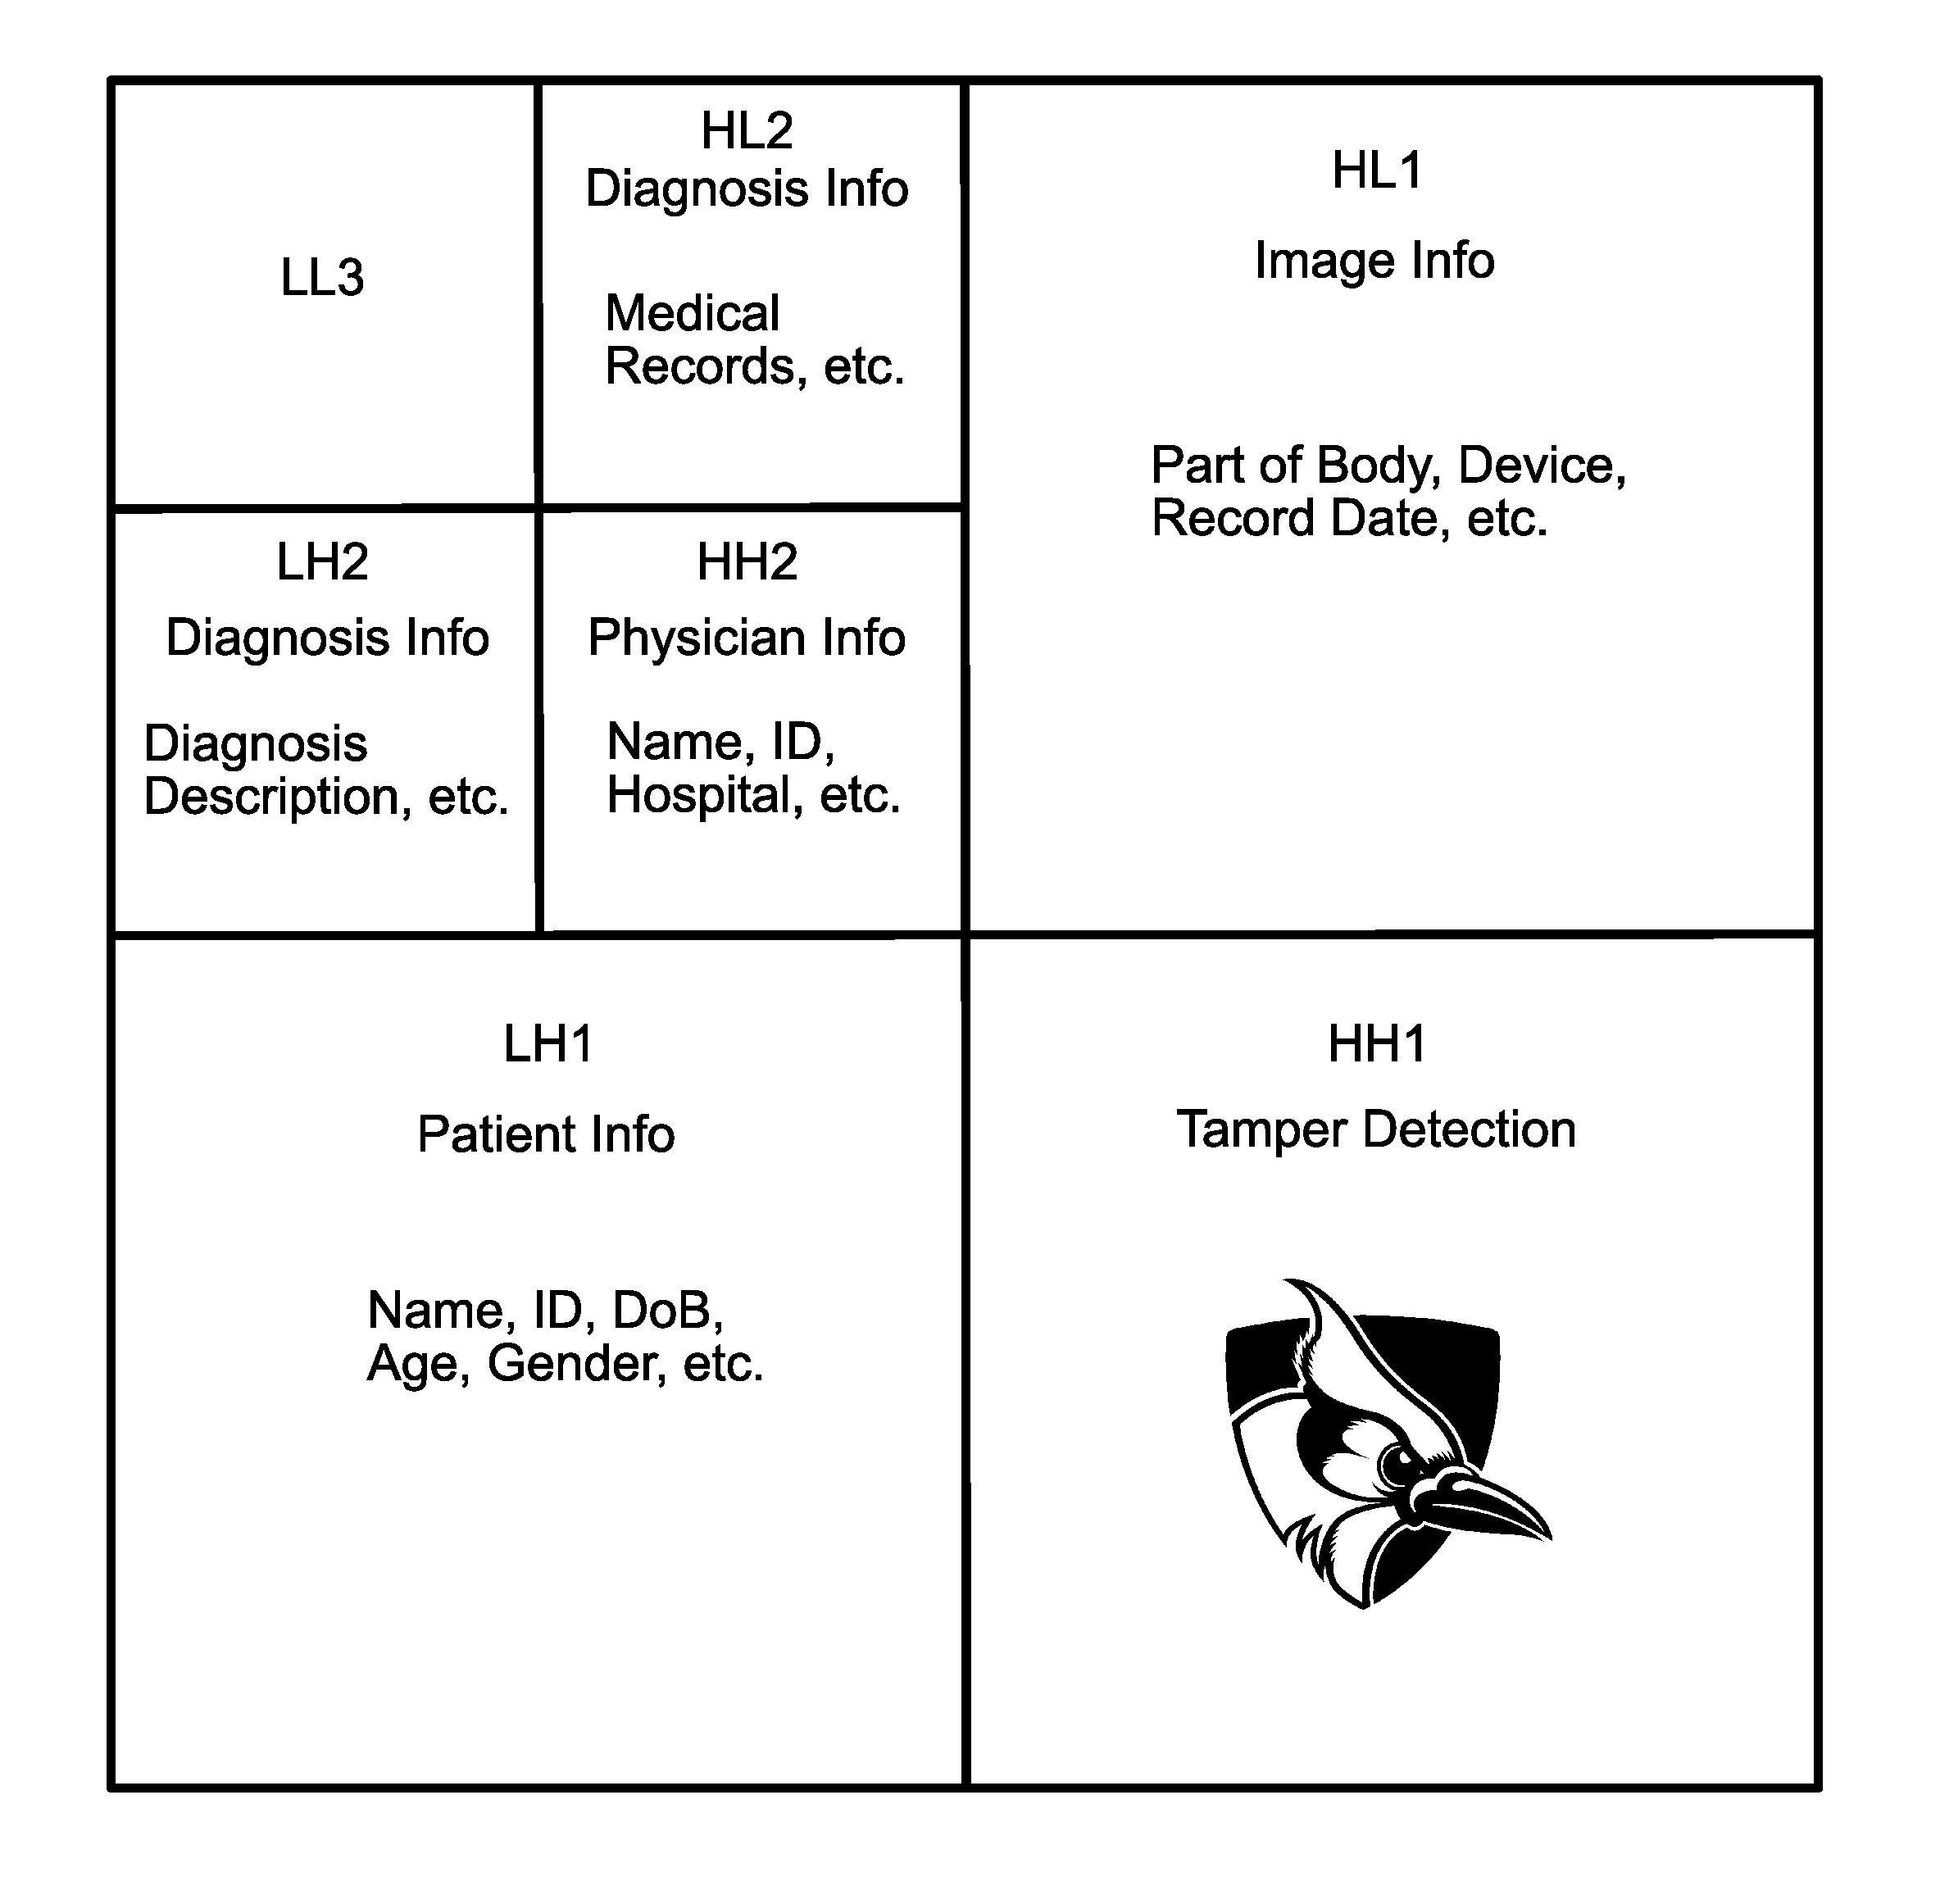
\includegraphics[width=1\linewidth]{WMPos}
	\caption{Structure of 2-level DWT and illustration of watermarking position}
	\label{WMPos}
\end{figure}
\\

\subsection{ROI segmentation}
In our scheme, ROI is defined by the lung area of CT image and we implemented zero watermarking to this part to achieve perfect reconstruction. The automated segmentation of ROI is based on the morphological reconstruction and the connected component analysis. We first applied the hole-filling algorithm to get the rough region of Lung and removed the false positives (like trachea, noise) according to the area of the connected components ($800 \leq N_{pixels} \leq100000$). The morphological close operation was performed to fill the gaps inside the lung region (Fig. \ref{ROI}). The ROI we acquire from segmentation would be used to specify the bitwise processing region in image based on the equation:
\[\ I_w = ROI^c \otimes Key\]
Where $I_w(x,y)\in\{0,1\}$ is an indicator of  the processed position. The corresponding watermarking position of level $L$ in wavelets domain can be determined by just down-sampling by $2^{L-1}$.
\begin{figure}[htbp]
	\centering
	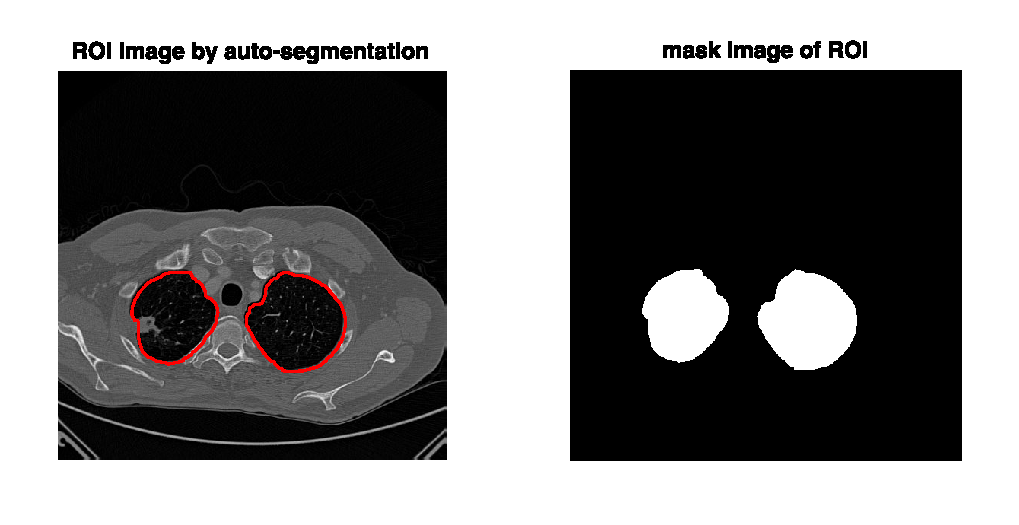
\includegraphics[width=1\linewidth]{ROI}
	\caption{Illustration of ROI in CT image. left: boundary of ROI. right: mask of lung region}
	\label{ROI}
\end{figure}
\\

\section{PERFORMANCE MEASURES}
We used four quality measures to evaluate our algorithm: signal-to-noise ratio, mean square error, peak signal-to-noise ratio and tamper assessment factor. Six common kinds of attacks in medical images were applied to test the watermarking performance.\\

\subsection{Signal-to-noise ratio (SNR)}
The SNR is used to estimate the noise of a signal in decibels. We take the original CT image as the signal and the deference between the processed image and the original one as the noise. SNR calculates the ratio of summed squared magnitude of the signal to that of the noise.
\[\ SNR(dB) = 10 log_{10} \frac{P_{Im}}{P_n}\]
Where $P_Im$ means the signal power and $P_n$ means the noise power.\\

\subsection{Mean squared error (MSE)}
The MSE is a measure of the quality of an estimator, which is defined as the average of the squares of the errors.
\[\ MSE = \frac{1}{M * N} \sum_{x=1}^{N}\sum_{y=0}^{M}(f(x,y)-Im(x,y))^2\]
Where $f(x,y)$ means the processed image, $Im(x,y)$ means the original image, $M$ and $N$ mean the width and the height of the image.\\

\subsection{Peak signal-to-noise ratio (PSNR)}
The PSNR is a ratio between the maximum possible power of a signal and the power of corrupting noise that affects the fidelity of its representation. PSNR is most commonly used in image reconstruction quality measurements, which is an approximation to human perception of image quality. PSNR is most easily defined via the MSE.
\[\ PSNR(dB) = 10 log_{10} \frac{MaxBits}{MSE}\]
Where $MaxBits$ stands for the maximum possible pixel value of the image.\\

\subsection{Tamper Assessment Factor (TAF)}
The TAF is an estimator of the error between the actual embedded watermark and the retrieved water mark. We embedded the known logo image into the diagonal detail of the first wavelet decomposition level and retrieved it. By calculating the deference between the actual watermark and the retrieved one.
\[\ TAF(w,w') = \frac{1}{M * N} \sum_{x=1}^{N}\sum_{y=0}^{M}(w(x,y)\oplus w'(x,y))\]
Where $w(x,y)$ means the original watermark, $w'(x,y)$ means the retrieved watermark, $M$ and $N$ mean the width and the height of the watermark image.\\

\section{RESULTS}

\section{FUTURE STEPS}


\addtolength{\textheight}{-12cm}   % This command serves to balance the column lengths
                                  % on the last page of the document manually. It shortens
                                  % the textheight of the last page by a suitable amount.
                                  % This command does not take effect until the next page
                                  % so it should come on the page before the last. Make
                                  % sure that you do not shorten the textheight too much.

%%%%%%%%%%%%%%%%%%%%%%%%%%%%%%%%%%%%%%%%%%%%%%%%%%%%%%%%%%%%%%%%%%%%%%%%%%%%%%%%



%%%%%%%%%%%%%%%%%%%%%%%%%%%%%%%%%%%%%%%%%%%%%%%%%%%%%%%%%%%%%%%%%%%%%%%%%%%%%%%%



%%%%%%%%%%%%%%%%%%%%%%%%%%%%%%%%%%%%%%%%%%%%%%%%%%%%%%%%%%%%%%%%%%%%%%%%%%%%%%%%
\section*{ACKNOWLEDGMENT}

SPIE-AAPM Lung CT Challenge

\begin{thebibliography}{99}
 \bibitem{c1} 
%\bibitem{c1} G. O. Young, ?Synthetic structure of industrial plastics (Book style with paper title and editor),? 	in Plastics, 2nd ed. vol. 3, J. Peters, Ed.  New York: McGraw-Hill, 1964, pp. 15?64.
%\bibitem{c2} W.-K. Chen, Linear Networks and Systems (Book style).	Belmont, CA: Wadsworth, 1993, pp. 123?135.
%\bibitem{c3} H. Poor, An Introduction to Signal Detection and Estimation.   New York: Springer-Verlag, 1985, ch. 4.
%\bibitem{c4} B. Smith, ?An approach to graphs of linear forms (Unpublished work style),? unpublished.
%\bibitem{c5} E. H. Miller, ?A note on reflector arrays (Periodical style?Accepted for publication),? IEEE Trans. Antennas Propagat., to be publised.
%\bibitem{c6} J. Wang, ?Fundamentals of erbium-doped fiber amplifiers arrays (Periodical style?Submitted for publication),? IEEE J. Quantum Electron., submitted for publication.
%\bibitem{c7} C. J. Kaufman, Rocky Mountain Research Lab., Boulder, CO, private communication, May 1995.

\end{thebibliography}


\end{document}
